\begin{figure}[h!]
  \centering
  \begin{tikzpicture}
    [spy scope= {circle, magnification=6, size=3cm},
      every spy on node/.style={draw, Red, thick},
      every node/.style={inner sep=0},
      label distance=-1cm]

    \node (original) {
      \begin{minipage}{0.45\textwidth}
        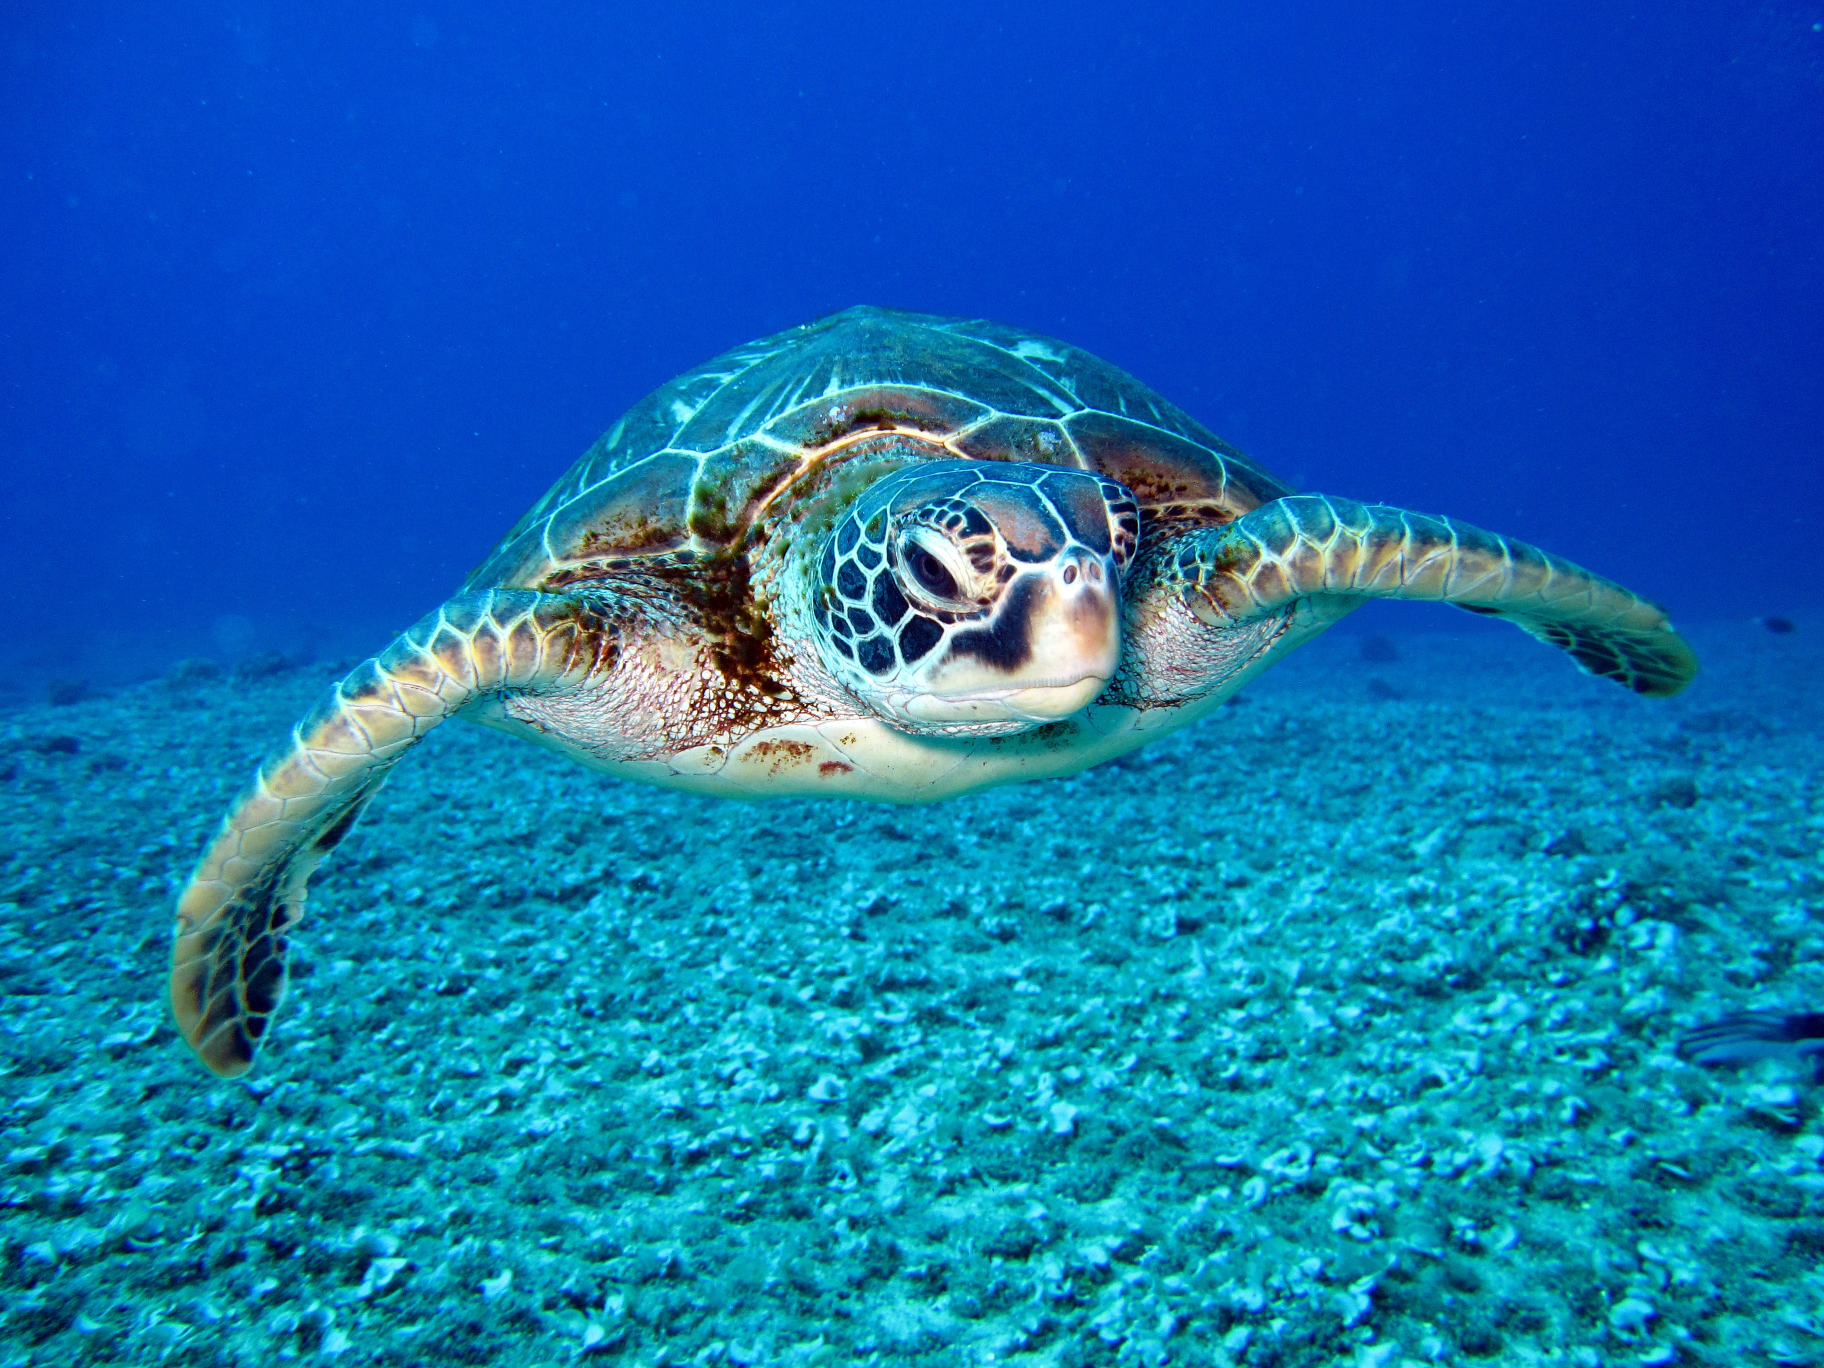
\includegraphics[width=1\textwidth]{turtle.png}
        \caption*{Original}
      \end{minipage}
    };
    \node [right= of original] (2mb) {
      \begin{minipage}{0.45\textwidth}
        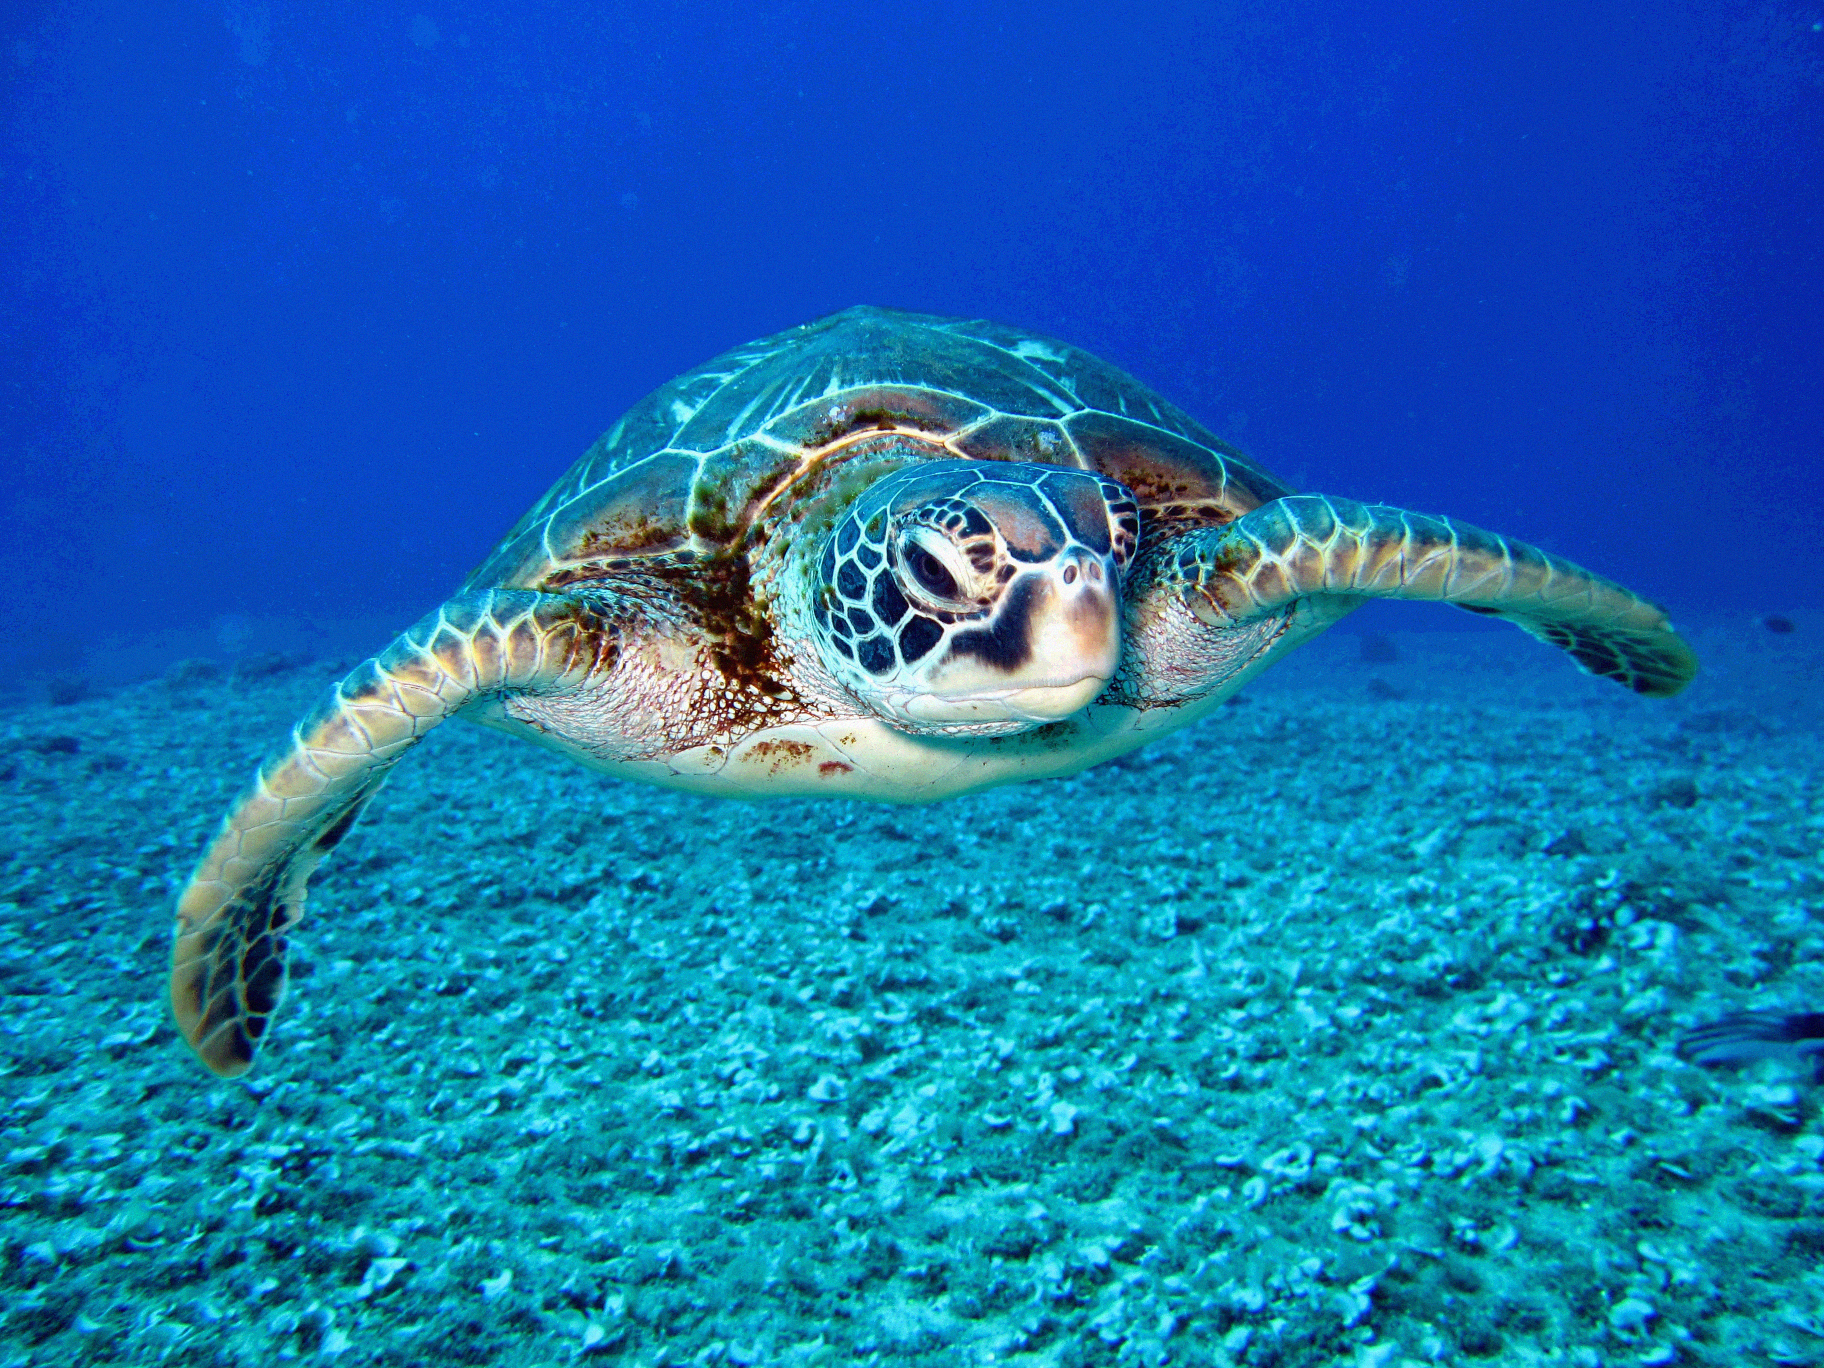
\includegraphics[width=1\textwidth]{turtle-3593134-48.png}
        \caption*{48\,\% (3,6\,MB)}
      \end{minipage}
    };
    \node [below=0.5cm of original] (4mb) {
      \begin{minipage}{0.45\textwidth}
        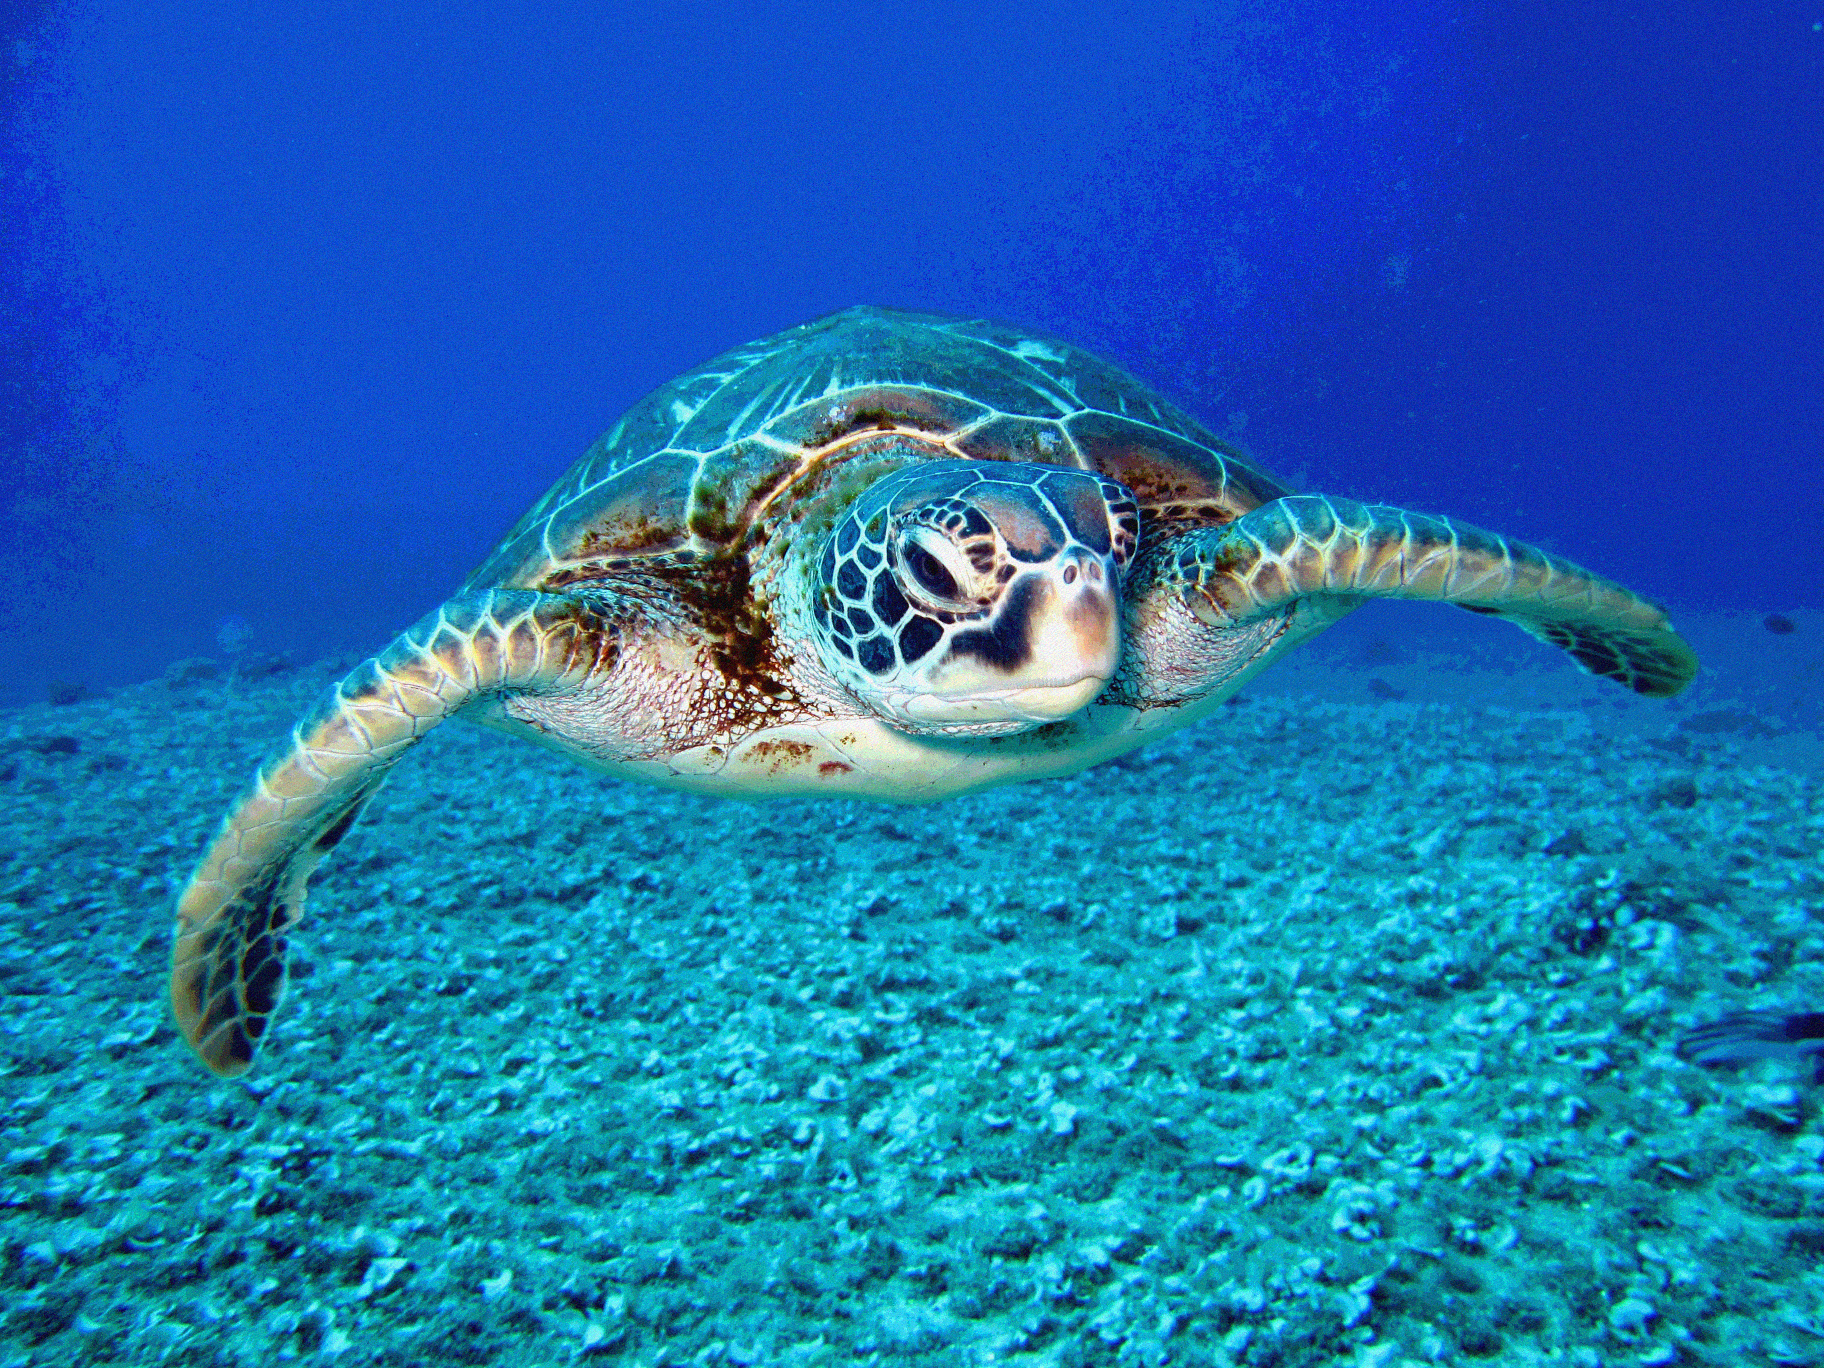
\includegraphics[width=1\textwidth]{turtle-4491417-60.png}
        \caption*{60\,\% (4,5\,MB)}
      \end{minipage}
    };
    \node [below=0.5cm of 2mb] (6mb) {
      \begin{minipage}{0.45\textwidth}
        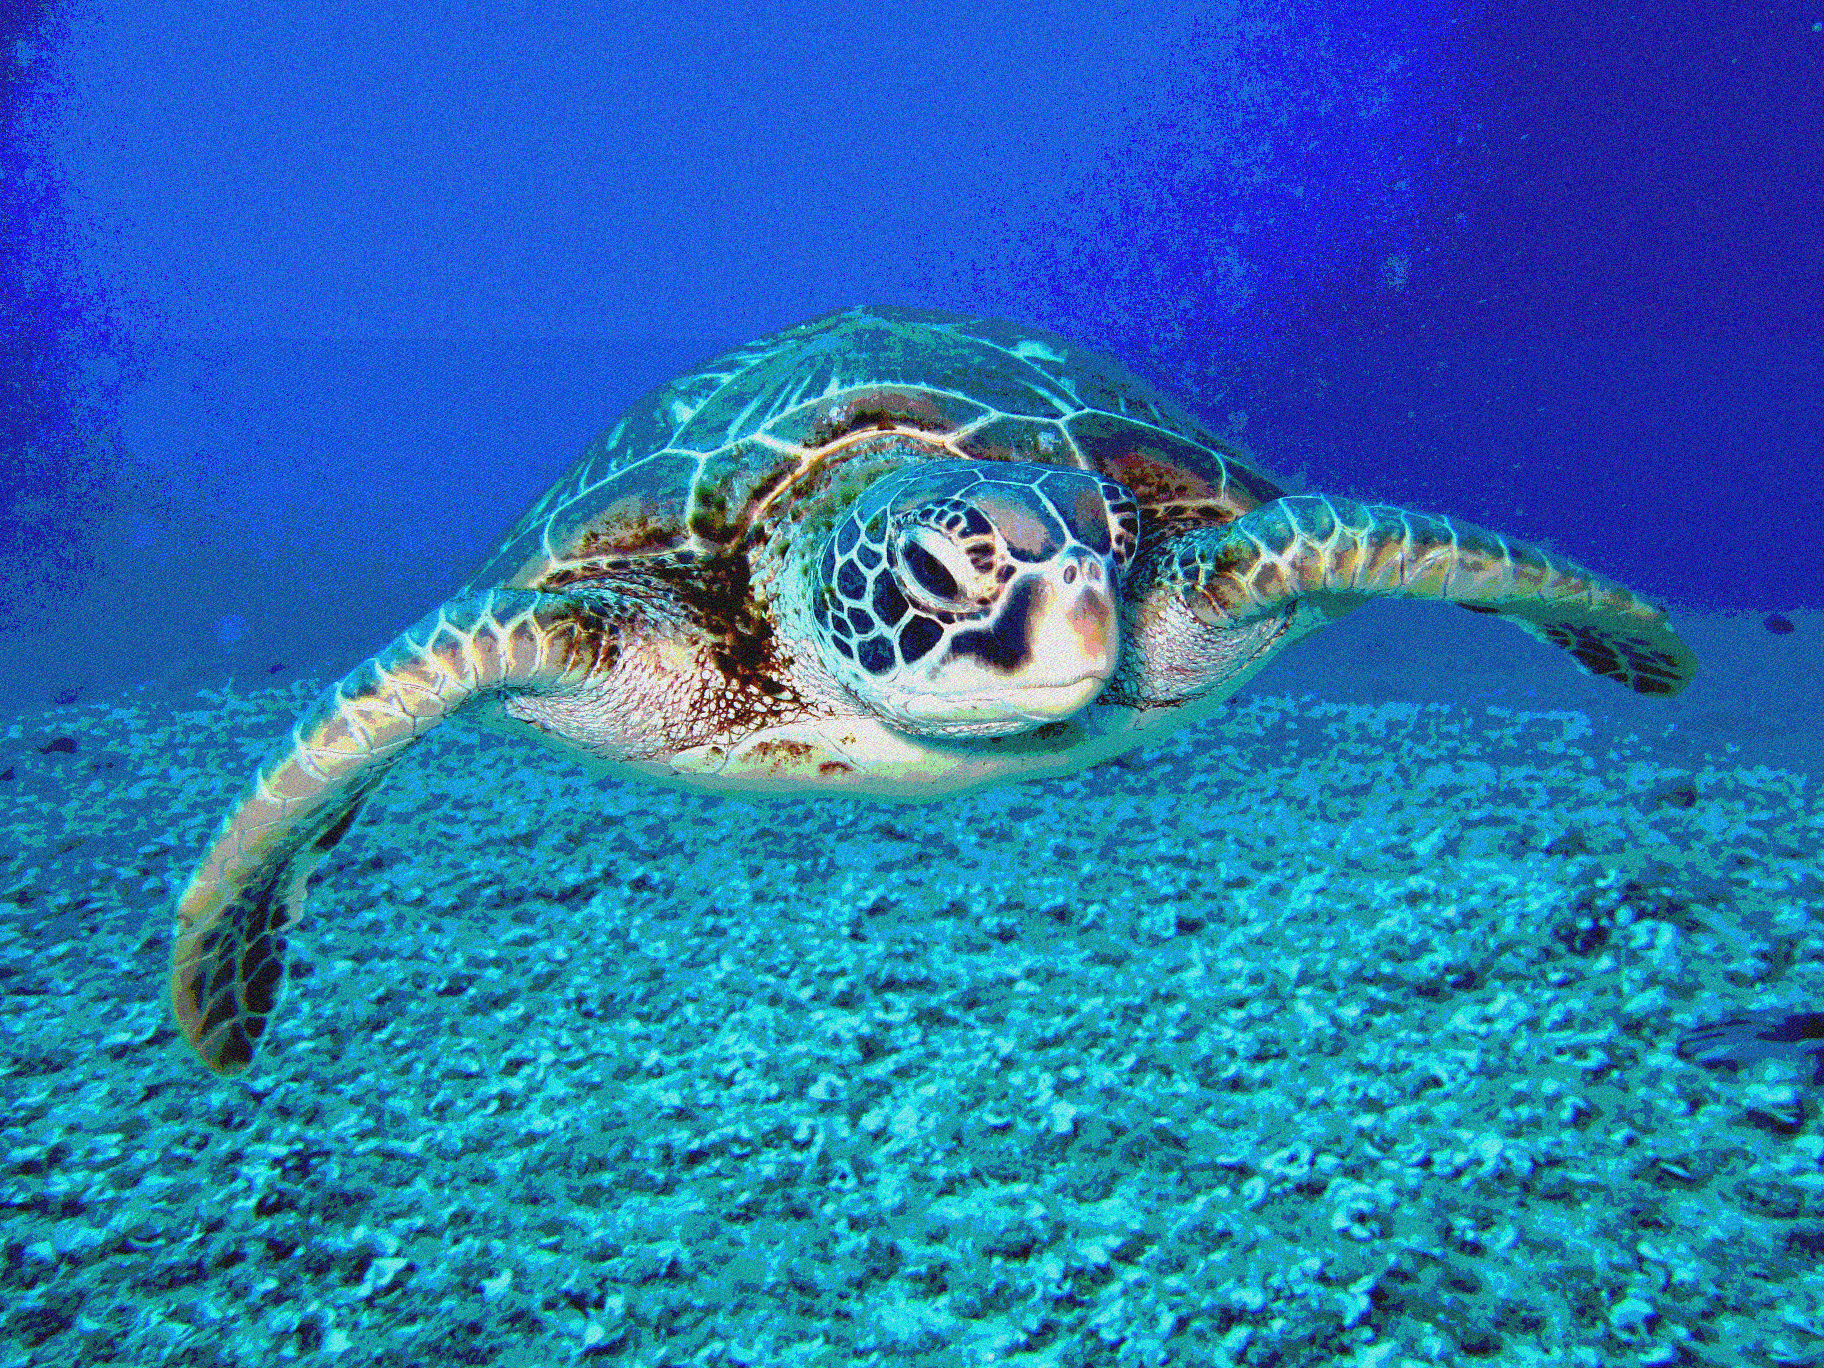
\includegraphics[width=1\textwidth]{turtle-5389701-72.png}
        \caption*{72\,\% (5,4\,MB)}
      \end{minipage}
    };

    \matrix [column sep=3.5cm] at ($(original.north)!0.5!(2mb.north) + (0,3.5cm)$) {
      \coordinate (a); & \coordinate (b); & \coordinate (c); & \coordinate (d); \\
    };

    \coordinate (spy-on) at (1.2cm,-0.6cm);

    \spy on ($(original.north) + (spy-on)$) in node[label=below:Original] at (a);
    \spy on ($(2mb.north) + (spy-on)$) in node[label=below:48 \%] at (b);
    \spy on ($(4mb.north) + (spy-on)$) in node[label=below:60 \%] at (c);
    \spy on ($(6mb.north) + (spy-on)$) in node[label=below:72 \%] at (d);


  \end{tikzpicture}
  \caption{Schildkröte. Größe 1368 $\times$ 1824 Pixel. Maximale Kapazität $\approx 7,5$\,MB.
    Gute Bildqualität bis zu 3,6\,MB versteckter Nachricht.}
  \label{fig:example-turtle}
\end{figure}
